\documentclass[10pt,a4paper]{article}
\usepackage{amsmath}
\usepackage{ctex}
\usepackage{graphicx}

\title{第二章 牛顿运动定律}
\author{华中科技大学大学物理A}
\date{2025.2.26}
\begin{document}
\maketitle
\section{notes}
牛顿第二定律$\vec{F}=\frac{d\vec{p}}{dt}$,
若质量不随时间变化\footnote{相对论中质量随速度变化}
,或$v<<c$则$\vec{F}=m\vec{a}$\\
常在分量上用牛顿第二定律.

\[\vec{F}=\frac{d\vec{p}}{dt}=\frac{d(m\vec{v})}{dt}
=m\frac{d\vec{v}}{dt}+\vec{v}\frac{dm}{dt}\]
万有引力$\vec{F}=-\frac{GMm}{r^{2}}\vec{e_r}$

质点系的牛顿第二定律(无质点或质量进出的情况)\\
对于单个质点:
\[\vec{F_i}+\vec{f_i}=\frac{d\vec{p_i}}{dt}=\frac{d(m_i\vec{v_i})}{dt}\]
累加得:
\[\vec{F_\text{合}}=\frac{d\vec{p_\text{合}}}{dt}\]
若每一质点速度相等,则$\vec{p_\text{合}}=m\vec{v}$,当$v<<c$时,
质点系有$\vec{F_\text{合}}=m\vec{a}$\\
若$\vec{F_\text{合}}$为变力,则$\vec{F_\text{合}}=m\vec{a}$为一微分方程.

\section{Exercises}
\subsection{课堂例题}
例1:一质量为$m$的物体在重力 的作用下以大小为$v_0$的初速度沿与水平方向成$\alpha$
角的方向向上抛出,空气阻力与物体动量成正比,
比例系数为$k(k>0)$,求物体运动轨迹.\boxed{\textbf{\text{建系}}}

建立$xOy$坐标系,分别在$x,y$方向上应用牛顿第二定律:
\[
\begin{cases}
-kmv_x=m\frac{dv_x}{dt}\\
-mg-kmv_y=m\frac{dv_y}{dt}
\end{cases}\Rightarrow
\begin{cases}
-kv_x=\frac{dv_x}{dt}\\
-g-kv_y=\frac{dv_y}{dt}
\end{cases}\Rightarrow
\begin{cases}
v_x=v_0\cos\alpha e^{-kt}=\frac{dx}{dt}\\
v_y=\frac{1}{k}[(g+kv_0\sin\alpha)e^{-kt}-g]=\frac{dy}{dt}
\end{cases}\]
\[
\Rightarrow
\begin{cases}
x=\frac{v_0\cos\alpha}{k}(1-e^{-kt})\\
y=\frac{1}{k^2}(g+kv_0\sin\alpha)(1-e^{-kt})-\frac{gt}{k}
\end{cases}
\]\underline{复习微分方程的解法!}

例2质量为$m$长为$l$的均质杆,绕端点$O$以角速度$\omega$
在光滑水平面上匀速转动,求杆中张力分布.
\begin{figure}[h]
\centering
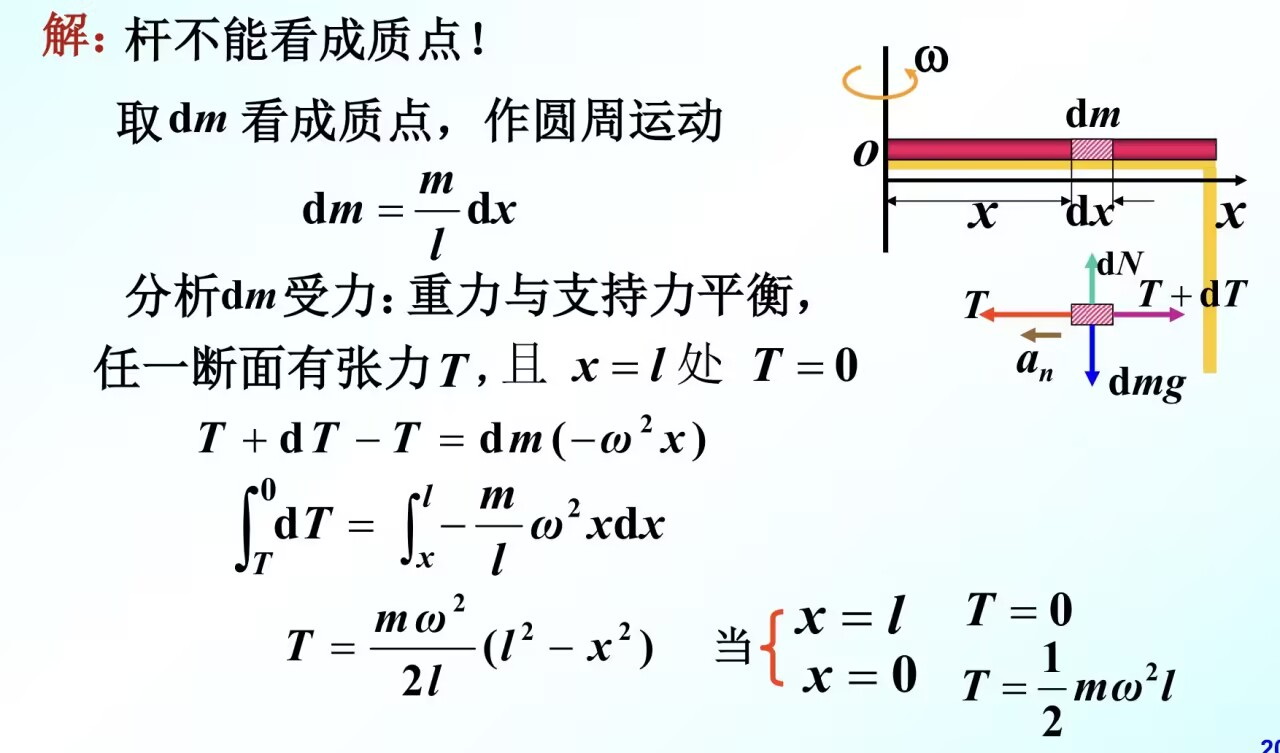
\includegraphics[width=0.8\textwidth]{eg2.jpg}
\end{figure}

例3
\begin{figure}[h]
    \centering
    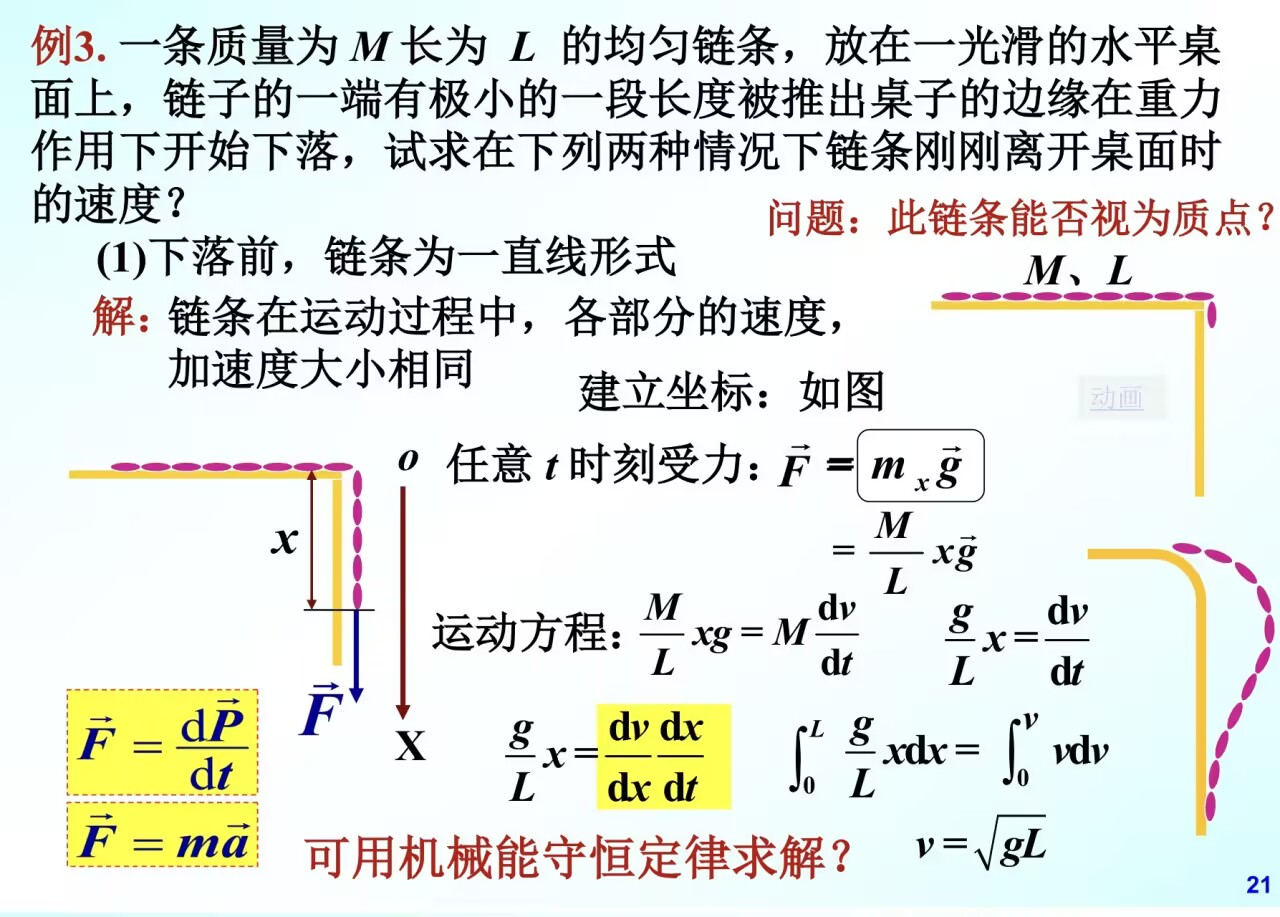
\includegraphics[width=0.8\textwidth]{eg3-1.jpg}
    \end{figure}
\newpage
例3情形2:
\begin{figure}[h]
    \centering
    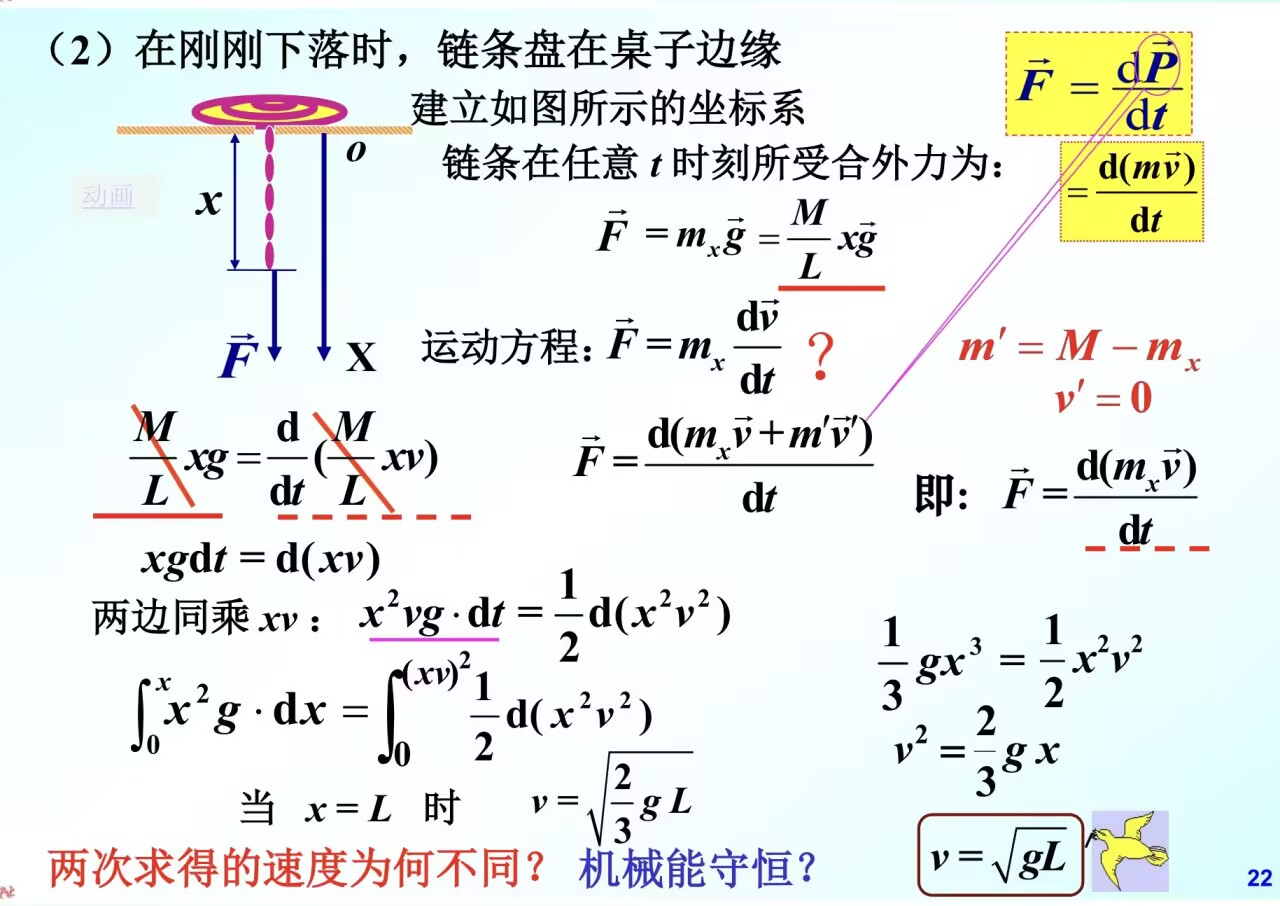
\includegraphics[width=0.8\textwidth]{eg3-2.jpg}
    \end{figure}

例4:
\begin{figure}[h]
    \centering
    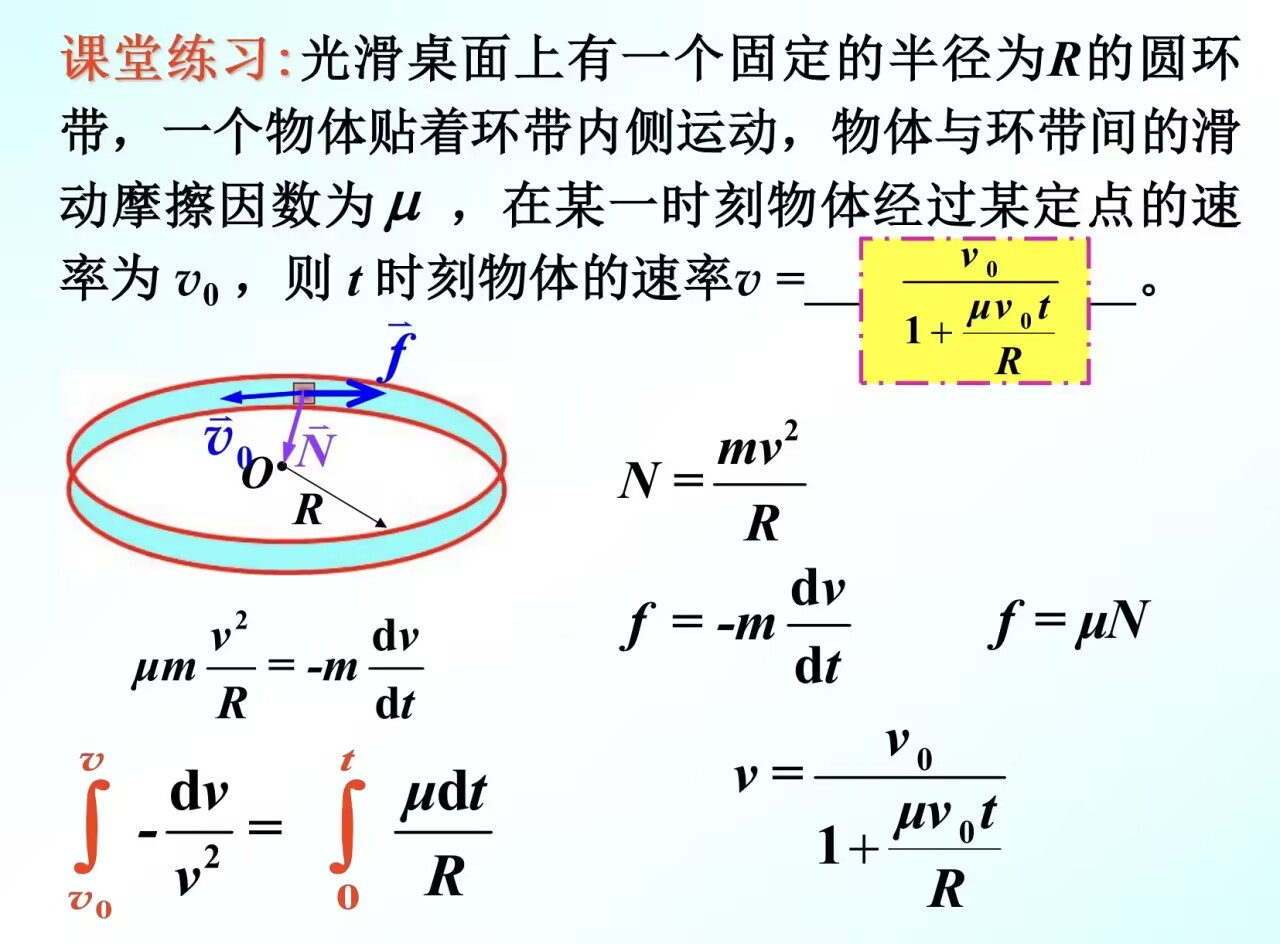
\includegraphics[width=0.8\textwidth]{eg4.jpg}
    \end{figure}
\end{document}